\documentclass[%
paper=a4,%
fontsize=11pt,%
twoside=false,%
DIV18,%
headsepline,%
plainheadsepline,%
footsepline,%
plainfootsepline,%
bibliography=totoc,%
listof=totoc,%
BCOR10mm,%
parskip=half,%
openany,%
]{scrartcl}
\usepackage[utf8]{inputenc}
\usepackage[english]{babel}
\usepackage{float}
\usepackage{graphicx}
\usepackage{color}
\usepackage{listings}
\lstset{basicstyle=\ttfamily\scriptsize}
\lstset{showspaces=false}
\lstset{showtabs=false}
\lstset{showstringspaces=false}
\lstset{keywordstyle=\bfseries}
\lstset{tabsize=4}
\lstset{frameround=ffff}
\lstset{extendedchars=true}
\lstset{stringstyle=\ttfamily}
\lstset{commentstyle=\ttfamily}
\lstset{backgroundcolor=\color[rgb]{0.92,0.92,0.92}}
%\lstset{numbers=left, numberstyle=\tiny, stepnumber=1, numbersep=5pt}
\lstset{captionpos=b}
\lstset{frame=single}
\setcounter{secnumdepth}{4} % Also numbering of \paragraph
\setcounter{tocdepth}{3} % Don't add \subsubsection to toc

% including and configuring package for links
\usepackage{hyperref}
\definecolor{darkblue}{rgb}{0,0,.5}

\hypersetup{pdftex=true, colorlinks=true, breaklinks=true, linkcolor=black, urlcolor=darkblue}

\title{Geany\LaTeX{} -- A \LaTeX{} plugin for Geany \\[1.5ex]
	   \normalsize Version 0.7}
\author{Frank Lanitz \\ \small{\href{mailto:frank@frank.uvena.de}{frank@frank.uvena.de}}}
\date{\today}

\newcommand{\up}[1]{\ensuremath{^\textrm{\scriptsize#1}}}

\begin{document}

\dedication{\normalsize \textbf{Note:} Please note that this document has been created on
\today. If you are using a devel version from GIT, please compile and check
\texttt{doc/geanylatex.tex} from sources. Please check Page \pageref
{sec:compiling_of_documentation}, Section \ref{sec:compiling_of_documentation} on how to do this. }


\pagenumbering{Roman}
\maketitle{}
\tableofcontents{}
\listoftables{}
\listoffigures{}
\lstlistoflistings{}

\newpage{}
\pagenumbering{arabic}
\section{About the plugin}

Geany\LaTeX{} is a little plugin to improve \LaTeX{} support in Geany.
It implements a couple of hopefully useful functions:

\begin{itemize}
	\item A wizard to create new \LaTeX{} documents in a fast and easy way
	 	  with a bunch of templates available
	\item A front end for adding labels \textbackslash label{} and
		  references \textbackslash ref{} and \textbackslash pageref{}
   		  getting suggestions from the document's aux file
	\item Insertion of special characters through the menu
	\item Help on BibTeX entries by templates and offering a list of
		  available references.
	\item Easy insertion of format patterns like \textbackslash texttt{}
		  through the menu
	\item Support of environment insertion by offering a dialog and
		  recognizing selections
	\item Shortcuts for inserting \textbackslash item and
		  \textbackslash newline
	\item Toolbar with frequently used format options
	\item A couple of useful auto-completion functions during typing
\end{itemize}

\newpage
\section{News \& ChangeLog}
\subsection{Geany\LaTeX{} 0.7 -- 2012-07-08}
\begin{itemize}
	\item Added a feature to lower selection before inserting
		\texttt{\textbackslash{}textsc\{\}}
\end{itemize}
\subsection{Geany\LaTeX{} 0.6 -- 2011-10-15}
\begin{itemize}
	\item Moved \LaTeX{} menu to a separate menu inside Geany main menu
	\item Added a feature to autocapetlise letters on typing on begin of
		  a sentence
	\item Added a way to put a icon for \LaTeX{}-wizard into Geany's main
		  toolbar
	\item Added a dialog for inserting BibTeX references based on
		  available *.bib-files
	\item Upgrade plugin API to version 199
\end{itemize}

\subsection{Geany\LaTeX{} 0.5 -- 2010-06-13}
\begin{itemize}

	\item Introduced custom templates for \LaTeX-Wizard
	\item Added a \LaTeX-Wizard icon to the toolbar
	\item Added shortcuts for inserting common list environments
		  like \texttt{enumerate}, \texttt{itemize} and
		  \texttt{description}
	\item Some general bugfixes and improvements. As always, see the
		  ChangeLog or svn log.
	\item Switched to waf for building the plugin
	\item Moved some \LaTeX{}-specific stuff out of Geany's core into the
		  plugin. This affects features like
			\begin{itemize}
				\item Autocompletion of \texttt{\textbackslash{}end\{\}}
					and \texttt{\textbackslash{}endgroup\{\}}
			\end{itemize}
	\item Proceeded to Geany Plugin API v184
	\item Made reference insertion configurable.
	\item Added an function to insert \textbackslash{}usepackage\{\} into
		  header of file
	\item Automatic adding of \{\} after typing of \_{} and \symbol{94}
	\item Added automatic inserting of \{\} after typing a command and
		  hitting return in case of none pair is already present

\end{itemize}

\subsection{Geany\LaTeX{} 0.4 -- 2009-05-26}
\begin{itemize}
	\item Added a toolbar with frequently used format commands
	\item Added a configuration dialog to configure basic options
          of the plugin
	\item Moved documentation into a \TeX{}-document
	\item Replace \textbackslash{}u-UTF-8 letters by octal coded
          chars to avoid dependency on C99.
	\item Added a function to bulk replace special characters
          inside marked text by keybinding
	\item Added a function for special characters substitution during typing
\end{itemize}

\newpage
\section{Requirements}

\small{\textbf{Please note:} This section of documentation is only
valid with standalone distribution of Geany\LaTeX{}. If you are
planning to use the common geany-plugins project, please check
documentation over there as there are some specialties you might
like to know.}

For compiling the plugin yourself, you will need the GTK ($>= 2.8.0$)
libraries and header files. You will also need its dependency
libraries and header files, such as Pango, Glib and ATK. All these
files are available at \url{http://www.gtk.org}.

And obviously, you will need to have Geany with its header files
installed (in case you are compiling the plugin on your own). If you
installed Geany from the sources, you should be ready to go. If you
used a prepared package, e.g. from your distribution, you probably
need to install an additional package, probably called geany-dev or
geany-devel. Please note that in order to compile and use this
plugin, you need Geany 0.21 or later (Geany Plugin API v199 or
higher).

Furthermore you need, of course, a C compiler and python installed.
The GNU version of the C compiler is recommended. Furthermore, there
should be a working \LaTeX-environment on your System.

There is no special need in RAM or CPU, so the plugin should compile
and run on all systems Geany is able to run.

\section{Compiling}
\subsection{Compiling the plugin}
For documentation how to compile the plugin, please check the
documentation of the geany-plugins combined release.
\subsection{Compiling the documentation}
\label{sec:compiling_of_documentation}
Sources of this documentation are available throught
\texttt{doc/geanylatex.tex} inside source tree. To compile the sources,
usage of \texttt{pdflatex} (should be delivered with your favorite
\LaTeX{} distribution) is recommended. For compiling into HTML format you
might like to use \texttt{htlatex}. The HTML version of this documentation
shipped with source tarball has been compiled with:

\begin{lstlisting}[caption={Compiling of documentation}]
htlatex geanylatex.tex xhtml -cvalidate -interaction=batchmode
\end{lstlisting}

\texttt{htlatex} most likely can be found in a package called \texttt{tex4ht}
-- At least it's called like that on Debian based operating
systems.

\section{Usage}
\begin{figure}[h!]
	\centering{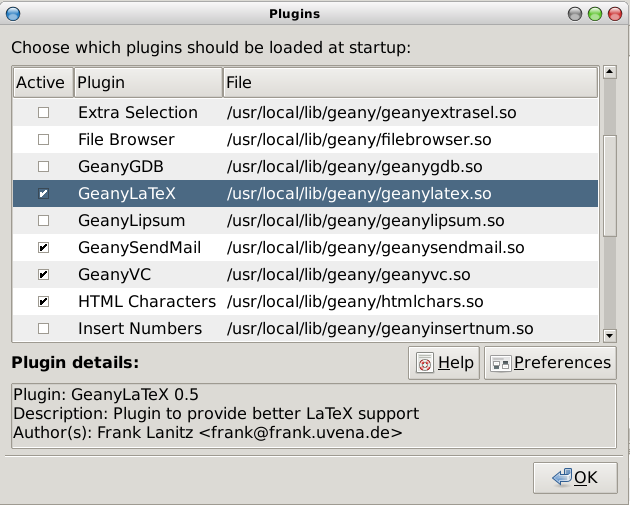
\includegraphics[height=7cm]{img/plugin_manager.png}}
	\caption{Plugin manager with Geany\LaTeX{} 0.5 at Geany 0.19}
\end{figure}

After Geany\LaTeX{} has been installed successful the plugin can be
loaded through Geany's plugin manager. Depending on configuration a
new menu inside Geany's main menu will appear, an menu entry for the
\LaTeX{}-wizard will appear inside the Tools menu as well as new key
bindings will be available inside Geany's key binding interface.
Inside the new menu you will find entries for functions supported by
this version of the plugin. The main menu entry will be called
something like \texttt{LaTeX}, depending on your locale.

Also if the option for showing the toolbar is activated on configuration
dialog, the toolbar with common used format functions appears on at top
of editor widget. This feature is turned off by default.


\section{Features}

Let's go into more detail on some features.


\subsection{\LaTeX-Wizard}

\subsubsection{General usage of wizard}
The \LaTeX-Wizard is implementing a easy way creating a number of
default documents.
\begin{figure}[h!]
	\centering{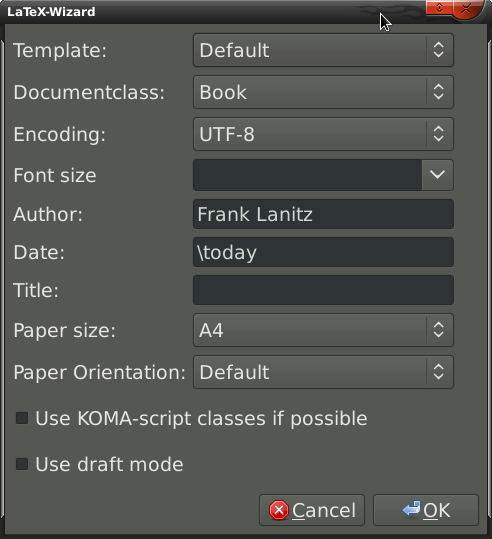
\includegraphics[height=7cm]{img/latexwizard.png}}
	\caption{\LaTeX-Wizard of version 0.5}
\end{figure}

The wizard is offering a chance to choose from a couple of templates
with the possibility of adding customer templates. This can be
chosen from \textbf{Templates} pulldown on top of dialog.

This can be set by choosing the needed entry form
\textbf{Documentclass} pulldown menu.

\textbf{Encoding} is configuring the packages \texttt{inputenc} to
for example \texttt{\textbackslash usepackage[utf8]\{inputenc\}} in
case of the document encoding should be UTF-8. Also it sets the
encoding Geany is using for the newly created document.

\textbf{Font size} as well as \textbf{Paper size} will set class option
for font/paper size of the new created document. \textbf{Author},
\textbf{Date}, \textbf{Title} will be also passed to the corresponding
command inside the file header.

Option \textbf{Use draft mode} will add \texttt{draft} to list of
document options which allows some help during debugging of document.

Since KOMA script is quiet popular the option \textbf{Use KOMA script
if possible} allows to activate the usage of KOMA script. If this
options is activated instead of \texttt{book}, \texttt{scrbook} will
be used as document class. Default is activated here. This option is
deactivated by default and can be set through Geany\LaTeX{}'s
configuration dialog mentioned earlier in this document.

This wizard can also be called by a shortcut. Please have a look onto
Section \ref{kb_latex_wizard}, page \pageref{kb_latex_wizard}.

\subsubsection{Default templates}
Document types that are currently supported by the wizard are:
\begin{itemize}
	\item book
	\item report
	\item article
	\item letter (default letter class)
	\item presentation (\LaTeX{} beamer)
\end{itemize}

\subsubsection{Extending by own templates}
\label{sec:extending_wizard_by_own_templates}
Geany\LaTeX{} is offering a way for extending the wizard by user
defined templates. This templates will be stored inside the plugin
configuration dir with file extension glt. For creating a
customized template you will need to create a normal *.tex file and
store it inside the directory. On most Linux systems this should be
\texttt{\textasciitilde/.config/geany/geanyLaTeX/}.

Inside your template you can refer to wizard's field by using some
special strings which are:

\begin{table}[H]
\centering
\label{tab:symbols_in_custom_templates}
\caption{List of available symbols on custom templates}
\begin{tabular}{l|p{10cm}}
\textbf{Symbol} & \textbf{Usage}\\ \hline
\texttt{\{CLASSOPTION\}} & Will be replaced by the classoptions set on
	the wizard as for example font size or paper size.\\
\texttt{\{DOCUMENTCLASS\}} & Will be replaced by the choosen document
	class based on the pulldown of wizard and whether option for KOMA
	script has been set. \\
\texttt{\{DATE\}} & Will be replaced by the input given on the date
	field of wizard.\\
\texttt{\{TITLE\}} & Will be replaced by the input given on the title
	field of wizard.\\
\texttt{\{AUTHOR\} }& Will be replaced by the input given on the author
	field of wizard.\\
\texttt{\{ENCODING\}} & Will be replace by choosen encoding from pulldown
	of wizard\\
\texttt{\{OPENING\}} & Will be replaced by »Dear Sir or Madame« in local
	geany\LaTeX{} is running with. If you like to overwrite it, please
	don't use the symbol and hardcode the phrase instead.\\
\texttt{\{CLOSING\}} & Will be replaced by »With kind regards« in local
	geany\LaTeX{} is running with. If you like to overwrite it, please
	don't use the symbol and hardcode the phrase instead.\\
	\end{tabular}
\end{table}

If you have other than the default templates defined they will be
add to templates pulldown. So when creating a template, please keep
care to set up a good name for the file, as the filename will be
the identifier you can choose from on pulldown.

In future a number of templates should be available also online at
\url{http://frank.uvena.de/files/geany/data/geanyLaTeX/}. Please
feel also free to publish templates in case of you have some useful
one.

If you need more general templates, you may have a look onto Geany's
build in template feature -- briefly introduced on Chapter \ref
{sec:recommended_things_geany_template_system}, page \pageref
{sec:recommended_things_geany_template_system}.

\subsection{Inserting References and Labels}
An often used feature on writing of documents is adding and referring
to labels. Geany\LaTeX{} is adding some support here for more
comfortable adding new labels and reference offering a GUI.

\begin{figure}[h!]
	\centering{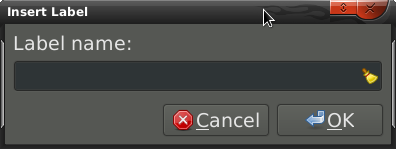
\includegraphics[height=2.5cm]{img/insert_label.png}}
	\caption{Insert label dialog on Geany\LaTeX{} 0.5}
\end{figure}

After an label was added Geany\LaTeX{} is offering a dialog for
inserting normal references and page references to a label.

\begin{figure}[h!]
	\centering{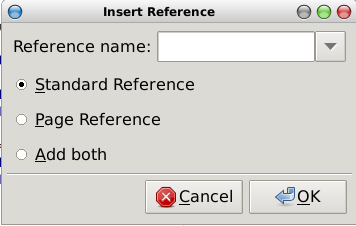
\includegraphics[height=3.5cm]{img/insert_reference.png}}
	\caption{Insert reference dialog on Geany\LaTeX{} 0.5}
\end{figure}

The suggestions inside the pull down are based on the aux files
creating by processing of *.tex file located inside directory of
current \TeX-file. When first step was successful the files are
parsed for \texttt{\textbackslash newlabel\{\}\{\}\{\}} and outcome
is tried to interpret them properly. The found entries will be
inserted into pull down sorted by alphabet.

Both, the inserting labels as well as the inserting reference dialog
can be accessed by key binding also. See Chapter \ref
{kb_insert_label} here.

\subsection{Support for BibTeX}
\subsubsection{BibTeX templates for catalogue entries}
Geany\LaTeX{} is offering a number of often used templates for BibTeX
catalogue entries. They can be access by the plugin submenu in Geany's
tools menu:
\begin{itemize}
	\item Article
	\item Book
	\item Booklet
	\item Conference
	\item Inbook
	\item Incollection
	\item Inproceedings
	\item Manual
	\item Mastersthesis
	\item Misc
	\item PhdThesis
	\item Proceedings
	\item Techreport
	\item Unpublished
\end{itemize}
When choosing an entry from list on menu a templace with common used
fields will be generated and inserted into the document.
The template will be inserted on position of cursor which will
no be moved during the process. As an example for a book, this will be
inserted to the document:

\begin{lstlisting}[caption={Example of BibTeX entry for a book}]
@Book{
Author = {},
Editor = {},
Publisher = {},
Title = {},
Year = {},
}
\end{lstlisting}


\subsubsection{Inserting cite-reference}

Geany\LaTeX{} is searching here for *.bib-files inside the directory
of current active file. Its filtering for all references inside
these files and putting it sorted and cleared from duplicated
entries into the pulldown of the dialog.

\begin{figure}[h!]
	\centering{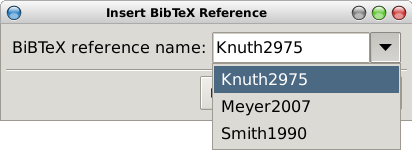
\includegraphics[height=2.5cm]{img/bibtex_reference.png}}
	\caption{Insert BibTeX reference dialog on Geany\LaTeX{} 0.6}
\end{figure}

With selecting one of the entries inside the pull down or by typing
in your own reference name, pushing enter or hitting OK will insert
a \texttt{\textbackslash{}cite\{\}} into your document with your
given reference.

\subsection{Replacement of special characters}
Geany\LaTeX{} is able to replace special characters to their there \TeX\
substitute. This can be done in two different ways:

\begin{enumerate}
	\item \textbf{On input:} If this switch is active all special
		  characters will be replaced during typing of text. You can
		  turn the switch on/off at Replacement of special characters
		  submenu inside.
	\item \textbf{Bulk replace of selected text:}
		  A selected text will be parsed and all known special characters
		  will be replaced by their \TeX{} substitute. This can be very useful
		  on importing a large amount of text into your document
		  including characters like ö or \frqq. This function is
		  available through the Replacement of special characters
		  submenu on plugin's submenu of Geany's Tools menu.
\end{enumerate}

For both functions there are also shortcuts available.

\subsection{Inserting of special character}
The plugin is offering a number of special characters with their \TeX{}
substitutes to be inserted on easy accessing through the plugin menu.

\subsection{Inserting of Environment}
Geany\LaTeX{} is offering a feature for inserting environments into your
documents. It can be chosen from a pulldown menu and will be inserted at
current position of cursor. If there is a selection activ, the selection
will be included into environment.

\begin{lstlisting}
\begin{your_environment}
	... selected text ...
\end{your_environment}
\end{lstlisting}

In case of an empty (= no selection) an empty environment with

\begin{lstlisting}
\begin{your_environment}
...
\end{your_environment}
\end{lstlisting}


will be inserted to the document.

\begin{figure}[h!]
	\centering{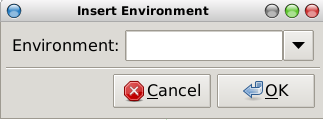
\includegraphics[height=2.5cm]{img/insert_environment.png}}
	\caption{Insert environment dialog on Geany\LaTeX{} 0.5}
\end{figure}


\subsection{Format}
Geany\LaTeX{} is able to help on formation of text. For doing this its
offering you to insert often use format patterns to your document.
Patterns that are currently supported are:

\begin{itemize}
	\item Italic
	\item Boldfont
	\item Underline
	\item Slanted
	\item Typewriter
	\item Small Caps
	\item Emphasis
	\item Centered
	\item left-aligned
	\item right-aligned
\end{itemize}

Geany\LaTeX{} will add the correct format pattern to the document. If
there is an selection active, that pattern will be placed around so
the selected text will be formatted with this chosen style.

Following items are also accessible using the Geany\LaTeX{} toolbar:
\begin{itemize}
	\item Italic
	\item Boldfont
	\item Underline
	\item Centered
	\item left-aligned
	\item right-aligned
\end{itemize}

\subsection{Autocompletion of \textbackslash{}begin and
  \textbackslash{}begingroup}

Since version 0.5 GeanyLaTeX{} is supporting autocompletion for
closing \textbackslash{}end and \textbackslash{}endgroup for begin
commands. Before Geany 0.19 this has been part of the Geany core
but has been moved out as it is something \LaTeX{} specific.

\subsubsection{Usage of feature}

After the feature has been enabled (Please check \ref
{sec:modus_of_autocompletion}, page \pageref
{sec:modus_of_autocompletion} here for more detailed information),
in every case you enter a \texttt{\textbackslash{}begin\{\}} or
\texttt{\textbackslash {}begingroup\{\}} the plugin will
automatically add the fitting \texttt{\textbackslash{}end\{\}} or
\texttt{\textbackslash{}endgroup\{\}} if its not finding a closing
tag within the definded context length -- by default this means
inside following 5 lines. If you like to change this size, please
check Chapter \ref {sec:hidden_pref_autocompletion_context}, page
\pageref {sec:hidden_pref_autocompletion_context}.

This feature is by default file type depending, so it will only work
on \TeX{}-like file types as well its turned on by default.


\subsection{Inserting \textbackslash{}usepackage\{\}-entry to header}

From time you need to insert a new package into header of a document,
but don't want to change to top of document and scroll back to where you were.

Since version 0.5 Geany\LaTeX{} is offering an easy to use dialog
which is taking over the package name and possible package options to
insert them into header of document. Right now, its placed direct in
top of the \texttt{\textbackslash{}begin\{document\}} statement if
there is any.

\begin{figure}[ht]
	\centering
	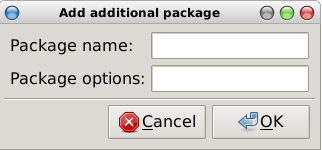
\includegraphics[width=0.4\textwidth]{img/insert_usepackage.png}
	\caption{Dialog for inserting \textbackslash{}usepackage\{\}}
\end{figure}

\subsection{Lower selection before inserting \textbackslash{}textsc\{\}}

With this feature, converting a normal text to \LaTeX{} is getting a
bit easier. If you start a document as plain text, with
abbreviations in it like ABC. You import it into \LaTeX{}, and want
the abbreviations in small caps. Geany\LaTeX{} converts the
selection to just use lower case letters. So \texttt{ABC} is
becoming \texttt{\textbackslash{}textsc\{abc\}} and later \textsc
{abc}. This can be configured via the plugin configuration dialog
and default value is turned off.

\section{Configuration}

GeanyLaTeX{} can be configured in three major ways:
\begin{enumerate}
\item GeanyLaTeX{}'s configuration dialog (see chapter \ref{sec:configuration_dialog},
	page \pageref{sec:configuration_dialog})
\item Geany's keybindings interface (see chapter \ref{sec:key_bindings},
	page \pageref{sec:key_bindings})
\item By hidden preferences which needs to be configured directly inside
	  configuration file (see chapter \ref{sec:hidden_preferences},
	page \pageref{sec:hidden_preferences})
\end{enumerate}

\subsection{GeanyLaTeX{}'s configuration dialog}
\label{sec:configuration_dialog}
With version 0.4 the configuration dialog is offering two options which
can be changed:

\subsubsection{Use KOMA script by default}
KOMA script bei Markus Kohm is a very popular set of document classes
mainly used in Europe. With this option the default setting for e.g.
\LaTeX{}-Wizard can be configured\footnote{Currently only position where
this option is being used to be honest}. Option is turned off by default.

\subsubsection{Show extra toolbar}
Decides whether toolbar with some format icons should appear in the top
of editor widget. Option is turned off by default. Just give it a try.

\begin{figure}[h!]
	\centering{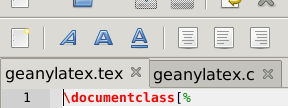
\includegraphics[height=2cm]{img/toolbar.png}}
	\caption{Plugin toolbar of Geany\LaTeX{} 0.5}
\end{figure}


\subsubsection{Capitalize letters on sentence begin}

If this option is enabled, Geany\LaTeX{} will look for \textsc{.},
\textsc{!} or \textsc{?} followed by a space. The next letter will
be inserted in capital letters. Currenty this is not working for
multichar letters as German Umlauts as well as the overwriting is
not supported very well at this point. In case of you don't want to
have the capital version of a letter in a particular case, just hit
undo (Ctrl + z in most cases).

\subsubsection{Add a wizard icon to Geany's main toolbar}
This adds an icon for Geany\LaTeX{} wizard to Geany's main toolbar
so its easy to access via mouse even the toolbar of Geany\LaTeX{} is
not active and the tools menu is a way to far away.

\subsubsection{Modus of autocompletion}
\label{sec:modus_of_autocompletion}
Here you can choose, whether the Geany\LaTeX{} should do some
autocompletion or not. Values are either
\begin{enumerate}
	\item Don't care about this inside plugin or
	\item Always perform autocompletion on LaTeX
\end{enumerate}

\subsection{Key bindings}
\label{sec:key_bindings}
Keybindings which are available:

\begin{table}[H]
\caption{List of available keybindings}
\centering
\label{kb_latex_wizard}\label{kb_insert_label}\label{kb_insert_reference}
\label{kb_toggling_input_replacement} \label{kb_replacement_of_special_char}
\begin{tabular}{l|p{9cm}}
\textbf{Shortcut} & \textbf{Description} \\ \hline\hline
Run LaTeX-Wizard & Starts the LaTeX-Wizard for creating a new document\\ \hline
Insert \textbackslash label & Runs the dialog for inserting a new label into your document. \\\hline
Insert \textbackslash ref & Starts an dialog for easy inserting \texttt{\textbackslash ref} and\texttt{\textbackslash pageref} into your document. The dialog is supporting easy parsing of aux files so it can suggest a couple of already set labels.\\\hline
Insert linebreak \textbackslash \textbackslash & Inserts a a newline \textbackslash{}\textbackslash{} into the document.\\\hline
Turn input replacement on/off & A shortcut for turning input replacement on or off. When input replacement is activated special characters like \v{e} are replaced by there \TeX{} substitute like \texttt{\textbackslash{}v\{e\}}\\\hline
Replacement of special characters & A selected text will be parsed and all known special characters
will be replaced by their \TeX{} substitute. This can be very useful on importing a large amount of
text into your document including characters like ö or \frqq. \\\hline
Run insert environment dialog & Runs a dialog for easy inserting an environment. If there is some text
selected, the environment will be placed around.\\\hline
Insert \textbackslash item & This shortcut will add an simple \textbackslash item to the document.
This can be very useful during writing of lists with a huge number of
items.\\\hline
Format selection in bold font face & Format a selection with bold font face.
This is done be adding \texttt{\textbackslash textbf\{...\}} around selection. \\\hline
Format selection in italic font face & Format a selection with italic font face.
This is done be adding \texttt{\textbackslash textit\{...\}} around selection.\\\hline
Format selection in typewriter font face & Format a selection with typewriter
font face. This is done be adding \texttt{\textbackslash texttt\{...\}} around
selection.\\\hline
Format selection centered & Formats selected text centered on page (uses \texttt{\textbackslash{}centering} \\\hline
Format selection left-aligned & Formats selected text left-aligned on page (uses \texttt{\textbackslash{}raggedleft} \\\hline
Format selection right-alignedm & Formats selected text right-aligned on page (uses \texttt{\textbackslash{}raggedright}\\\hline
Insert description list & Inserts an description environment as well as a 1\up{st} \textbackslash{}item element.\\\hline
Insert itemize list & Inserts an itemize environment as well as a 1\up{st} \textbackslash{}item element.\\\hline
Insert enumerate list & Inserts an enumerate environment as well as a 1\up{st} \textbackslash{}item element.\\\hline
Insert BibTeX reference dialog & Opens up a dialog which is supporting insertion of BibTeX-references based on \texttt{bib}-files inside current directory.\\\hline
Toggle autocompletion for \_ and \^ & Controlls whether braces should be inserted after \_ and \^ \ or not.
\end{tabular}
\end{table}


\subsection{Hidden preferencess}
\label{sec:hidden_preferences}
As not all users need to configure everything on there plugin, Geany
\LaTeX{} has some hidden preferences which can be set through
command line.

\subsubsection{Deactivate toolbar items if document is a non \TeX-type}
\label{deactivate_toolbaritems_with_non_latex}
By default, Geany\LaTeX{} is deactivating buttons inside toolbar, which
don't make much sense to be applied on non-\TeX{} file types. As
this is not always wished, its possible to turn this feature off
via a hidden preferences.

If you want to do so, just add a new section called \texttt{toolbar}
into your general.conf file of Geany\LaTeX{} plugin which stats
\texttt{glatex\_deactivate\_toolbaritems\_with\_non\_latex=false}.
As a result, your config file could look similar to this:

\begin{lstlisting}[caption={Configuration to enable toolbar buttons if %
						    no \LaTeX{} is active}]

[general]
glatex_set_koma_active=false
glatex_set_toolbar_active=true

[toolbar]
glatex_deactivate_toolbaritems_with_non_latex=false
\end{lstlisting}

Setting this option back to true will go back to default behaviour.

Please ensure, you reload the plugin once this option has been changed.

\subsubsection{Remove \LaTeX{} menu if document is a non \TeX-type}
\label{deactivate_menubarentry_with_non_latex}
Geany\LaTeX{} is enabling a separate menu inside Geany's main menu.
On default, its getting activated and deactivated based on the file
type of the current document. However, from time to time its annying
to have the menu entry switched maybe each time on switching between
two documents it can be set to keep even there is no LaTeX document
activ.

\begin{lstlisting}[caption={Configuration to keep \LaTeX{} menu inside menubar}]
[general]
glatex_set_koma_active=false
glatex_set_toolbar_active=true

[menu]
glatex_deactivate_menubarentry_with_non_latex=false
\end{lstlisting}

This option might make sense in combination with deactivation of
toolbar items on changing to a non-\TeX{} document at
\ref{deactivate_toolbaritems_with_non_latex}, page \pageref
{deactivate_toolbaritems_with_non_latex} set to \texttt{false}.

\subsubsection{Add \LaTeX{} menu on startup}

In case of you want to see always the \LaTeX{}-menu independent of
you have a \LaTeX{} document open. To add the menu direct at startup
time you might set \texttt{glatex\_add\_menu\_on\_startup} inside
menu section of configuration file to true.

\begin{lstlisting}[caption={Configuration add \LaTeX{} menu on startup of Geany}]
[general]
glatex_set_koma_active=false
glatex_set_toolbar_active=true

[menu]
glatex_deactivate_menubarentry_with_non_latex=false
glatex_add_menu_on_startup=true
\end{lstlisting}

This options makes only sense in combination with
glatex\_deactivate\_menubarentry\_with\_non\_latex
as described in chapter \ref{deactivate_menubarentry_with_non_latex},
page \pageref {deactivate_menubarentry_with_non_latex}.

\subsubsection{Size of context for autocompletion}
\label{sec:hidden_pref_autocompletion_context}
Inside configuration file you can add a value to adjust the size of
context, which is being searched for autocompletion of \texttt{
\textbackslash{}end} and \texttt{\textbackslash{}endgroup}. The
default value is 5. If you want to reset it, just add a new line to
your configuration file with
\texttt{glatex\_set\_autocompletion\_contextsize} followed by an integer
value. An example could look like this:

\begin{lstlisting}[caption={Example configuration for contextsize of autocompletion}]
[general]
glatex_set_koma_active=true
glatex_set_toolbar_active=false
glatex_set_autocompletion=true

[autocompletion]
glatex_set_autocompletion_contextsize=2
\end{lstlisting}

\subsubsection{Apply autocompletion only to \TeX{}-like files}
With this option, you can force Geany\LaTeX{} to apply all autocompletion functions also to non-\TeX{} file types as for example an C-source code file. As this is only in a very low number of cases a really good idea, the option is by default turned on.

\begin{lstlisting}[caption={general.conf example for deactivating file %
						   type specific restrictions for autocompletion}]
[general]
glatex_set_koma_active=true
glatex_set_toolbar_active=false
glatex_set_autocompletion=true

[autocompletion]
glatex_autocompletion_only_for_latex=false
\end{lstlisting}

\subsubsection{Customized reference strings}

Geany\LaTeX{} is able to insert references to a label where its
using some default value. As this value is not always optimal, it
can be changed using a hidden preference by setting
\texttt{glatex\_reference\_page}, \texttt{glatex\_reference\_chapter} or
\texttt{glatex\_reference\_all} inside configuration file as shown inside
the example configuration snippet.

\begin{lstlisting}[caption={Configuration example for customized reference strings}]
[general]
glatex_set_koma_active=true
glatex_set_toolbar_active=true

[reference]
glatex_reference_page=\\textbf{\pageref{{{reference}}}}
glatex_reference_chapter=\\textbf{\\ref{{{reference}}}}
glatex_reference_all=\\textbf{\\ref{{{reference}}}, page \pageref{{{reference}}}}
\end{lstlisting}

Please take care in this case \texttt{\{\{reference\}\}} will be
replace by label name.

Also \texttt{\textbackslash{}t}, \texttt{\textbackslash{}r},
\texttt{\textbackslash{}n} will be handled as known from C so you will
need to add a second \textbackslash{} in front of in such cases. Even
this seems to be annyoing on the first hand, it allows you to insert some
more complicated constructs over  here which might require a new line inside.


\subsubsection{Autocompletion of \{\} after \_ and \symbol{94}}
\label{sec:autoadding_of_braces}
Geany\LaTeX{} is able to autocomplete \{\} after typing \_ and
\symbol{94}. This might by useful on typing mathematic text and
formula. However, as this option is turn on by default and it might
get annoying you can deactivate it by setting \texttt{glatex\_set\_autobraces}
inside \texttt{[autocompletion]} section of configuration file. An example
which is turning off the feature might can look like this:

\begin{lstlisting}[caption={Configuration example for autocompletion of %
							\{\} after \_ and \symbol{94}}]
[general]
glatex_set_koma_active=true
glatex_set_toolbar_active=true
glatex_set_autocompletion=true

[autocompletion]
glatex_set_autobraces=false
\end{lstlisting}

\textbf{Note:} The feature in general is only working, if
\texttt{glatex\_set\_autocompletion=true} is also set to \texttt{true}.

\subsubsection{Autoadding of \{\} after a command}

The plugin can autoadd a pair of braces \{\} on hitting return after typing a
command. The function will search for a \textbackslash{} and will
stop once it founds a space, some \{\} or a second \textbackslash{}
as on \textbackslash{} \textbackslash{}. This can be configured also
by using the hidden preference \texttt{glatex\_set\_autobraces}
described in chapter \ref{sec:autoadding_of_braces}, page \pageref
{sec:autoadding_of_braces}.


\section{Contribution to the plugin}
If you like the plugin, there are a number of ways, how to
contribute to the development of the plugin.

\subsection{Extending plugin}

\subsubsection{Adding a new translation}
\label{sec:translating}
Currently the plugin is available in English and German language but
we are always looking for other translations to. There are two major
topics in translation:

\begin{enumerate}
\item \textbf{Translation of plugin:}
	   Adding a new translation and improving an existing one is easy to
	   do. After catching the source tarball and extracting you can find
	   all needed files inside the po/ folder. \\
	   Please contact the authors if you plan to update/add a translation
	   to ensure nobody else is currently working on and avoid double
	   work and to get some further information about translation (see
	   Chapter \ref{contact}).
\item \textbf{Translation of documentation:}
	   Since this document is currently only available in English it
	   would be helpful for not English speaking people to have a
	   translated version. If you like to do an translation, please
	   also contact one of the authors for details (see Chapter \ref{contact}).
\end{enumerate}

\subsubsection{Adding a new feature}
New features are always highly welcome. The TODO file inside source
code archive gives a good idea of current wished features and which
are being worked on. Also you can have a look onto the feature request
tracker of geany-plugins project at
\url{https://github.com/geany/geany-plugins/issues} whether you find
something interesting. Of course we are also open for not in the
sources mentioned before listed items. Just contact one of the authors
(see Chapter \ref{contact}).

When sending a patch which is adding a new feature, please check
whether you did also care about some documentation for it. As the
user will need some, it might can increase the speed a patch is
applied. Of course you should also check chapter \ref{sec:sending_a_patch},
page \pageref{sec:sending_a_patch} for maybe some more detailed
information before.

\subsection{Testing \& bug reporting} Geany\LaTeX{} is tested mainly
on x86 and x86\_64 architecture running GNU/Linux. Also it was
tested on some Windows 32 versions like XP SP3 very briefly. Since
there are also other systems available, testing on other platforms
and maybe reporting of issues is highly appreciate.

\subsection{Packaging}
Geany\LaTeX{} is part of the geany-plugins project even though there
are releases independent of a major release of the project. Therefor
there are two things you can do here:
\begin{enumerate}
	\item Package the plugin for your operating system or
	distribution. As you might can imagine, the authors unfortunately
	cannot support all possible platforms.
	\item Help to keep releases and packages of geany-plugins project
	up to date for current version of Geany.
\end{enumerate}


\subsection{Improving and extending of documentation}
Documentation is never complete. There are spelling mistakes,
paragraphs that needs to be extended or rewritten because they are not
clear or topics that were missed out at all.

The documentation is written in \LaTeX{} so all you need is to get the
tex file from doc folder and add or update the content.
After this, just send a diff or complete file to one of the authors.


\subsection{Providing additional data for plugin}

You can also contribute to the plugin's development by providing
additional data as for example customized templates for the
\LaTeX-Wizard. If you build up one, you might like to send it to
one of the authors.

\subsection{Propaganda}
And of course, tell others of Geany and this plugin. If you like to do
a talk about Geany\LaTeX{} and/or Geany in general, there is some code
available on \url{http://git.geany.org/talks/} you might can use as a
start point for preparing your own presentation. If your favourite
language is not yet available there, please feel free to do your own
translation and in best case send your translation to one of
Geany's\footnote{Check for addresses \url{http://www.geany.org}}
development team so it can be added to archive.


\section{Development}
\subsection{Development version}
You can checkout the current source code from the git-repository
at github.com. Get the code by clone the repository:

git clone https://github.com/geany/geany-plugins.git

\subsubsection{Sending a patch}
\label{sec:sending_a_patch}
If you want to create a patch, please respect the license of
Geany\LaTeX{} as well as intellectual property of third. Patches that
should be included to the default distribution must be licensed under
the same conditions as Geany\LaTeX{} by the copyright owner.

\section{Known issues}
At time of the the documentation was created no issue were known.
Since this is only a snapshot, you will find more recent information
for all reported issues bug tracking system of GitHub at \\
\url{https://github.com/geany/geany-plugins/issues}

\section{Recommendations to improve work with \LaTeX{} and Geany}
Geany is offering a number of nice features that can be used to make
daily work more easy without need to write a new plugin or extend
Geany\LaTeX{}.

\subsection{Geany's build system}

On Geany you can define a couple of commands for the build system to
improve work with your source file.

\subsubsection{Document backward search}
When working on a document it happens taht you find a typing error or
some more generic issue on your document. Once this happend, its hard
to find the correct position in your tex file. If you are using xdvi
you can use the backward search function to jump to the right place of
your document. An example configuration line for Geany's build system
could look similar to  this snippet:

\begin{lstlisting}
xdvi -editor "geany --line %l '%%f'" "%f"
\end{lstlisting}

\subsection{Geany's template system}
\label{sec:recommended_things_geany_template_system}
If you don't need a dynamic template as described in Chapter \ref
{sec:extending_wizard_by_own_templates}, page \pageref
{sec:extending_wizard_by_own_templates} you can also use Geany's
buildin template function which allows to also add customised
templates, including placeholders for e.g. author's name, but in a
more general and non\LaTeX{}-specific way. Nevertheless you should
give it a try as it is useful in many cases. For information on how to
create your own template using Geany's built-in feature, please
check the manual.

\subsection{Geany's code snippet function}
Geany allows you to define code snippets and re-insert them easily
at different places throughout your document.

A possible snippet for snippets.conf could be:

\begin{lstlisting}[caption={Minimal snippets.conf for \LaTeX{}}]
[LaTeX]
frame=\\begin{frame}\n%ws%\\frametitle\n%ws%%cursor%\n\\end{frame}
block=\\begin{block}\n%ws%%cursor%\n\\end{block}
itemize=\\begin{itemize}\n%ws%\\item %cursor%\n\\end{itemize}
enumerate=\\begin{enumerate}\n%ws%\\item %cursor%\n\\end{enumerate}
description=\\begin{description}\n%ws%\\item %cursor%\n\\end{description}
\end{lstlisting}

A snapshot of the authors' last version for LaTeX can be found on
\url{http://www.geany.org/Download/Extras}

\subsection{Other useful plugins}
As mentioned before, a number of useful functions are already
implemented in other plugins. Below you will find a list with the
authors's recommendations. More nice plugins can be found on Geany's
plugins page at \url{http://www.geany.org}.

\subsubsection{GeanyLipsum}
This plugin implements an easy way for inserting Lorem Ipsum text into
a document. The length of the inserted text if configurable so the
plugin can be very helpful on testing layout.\\
\textbf{Homepage:} \url{http://frank.uvena.de/en/Geany/geanylipsum/}

\subsubsection{geanyVC}
When working on bigger documents a version control system like
Subversion could be useful to keep versions. GeanyVC is adding a easy
to use frontend for a number of popular version controll systems such
as git, Subversion, CVS, Bazaar or Mercural.\\
\textbf{Homepage:} \url{http://plugins.geany.org/geanyvc/}

\subsubsection{Spellcheck}
Nobody is perfect - in special with typing mistakes on writing a
text. Spellcheck is offering a way on Geany to make usage of a
common spellchecking sytem as aspell, myspell or hunspell. Wrong
spelled words can be marked with an red line and the plugin is
offering suggestions for correct the word. Unfortunately right now
its not supporting some special things common in \TeX{} and \LaTeX{}.\\
\textbf{Homepage:} \url{http://plugins.geany.org/spellcheck/}

\subsubsection{tasks out of the addons plugins}
A plugin that is recognising \texttt{TODO} or \texttt{FIXME} tags
inside a document and allows to easy jump to these entries. This
function is similar to the \texttt{todo} package but doesn't require
recompiling of the document. Recognised tags will be inserted to
another tab in Geany's message widget.\\
\textbf{Homepage:} \url{http://plugins.geany.org/addons/}


\subsubsection{Tableconvert to convert a tabulator separated list into a table}

Its an quiet annyoing problem which happens from time to time: There
is a list of values e.g. from some experiment which needs to be
included into your document. The \LaTeX{}-export filter of your
spreadsheet tool is not very adavanced and you just want to insert a
couple of lines and have to do it manually.

Tableconvert is offering to convert a tabular separated list into an
table. The plugin is also offering to convert such a list into a
\LaTeX{}-like table and therefor is maybe useful on daily work.

\section{License}
Geany\LaTeX{} and all its parts is distributed under the terms of the
GNU General Public License as published by the Free Software
Foundation; either version 2 of the License, or (at your option) any
later version. A copy of this license can be found in the file COPYING
included with the source code of this program. If not, you will be
able to get a copy by contacting the Free Software Foundation, Inc.,
51 Franklin Street, Fifth Floor, Boston, MA 02110-1301, USA.


\section{Bugs, questions, homepage}
\label{contact}
If you found any bugs or want to provide a patch, please contact Frank
Lanitz (frank(at)geany(dot)org). Please also do so, if you got any
questions and visiting \\ \url{http://frank.uvena.de/en/Geany/geanylatex/}
didn't help you to figure out the answer. Visiting the website is also
a good start if you want to check for any update on this plugin.

\end{document}
